%%%%%%%%%%%%%%%%%%%%%%%%%%%%%%%%%%%%%%%%%%%%%%%%%%%%%%%%%%%%%%%%%%%%%%
%%%%%%%%%%%%%%%%%%%%%%%%%%%%%%%%%%%%%%%%%%%%%%%%%%%%%%%%%%%%%%%%%%%%%%
%%%%%%%%%%%%%%%%%%%%%%%%%%%%%%%%%%%%%%%%%%%%%%%%%%%%%%%%%%%%%%%%%%%%%%
\chapter{Redesign of differential equations}
\label{ch:DEs}

%%%%%%%%%%%%%%%%%%%%%%%%%%%%%%%%%%%%%%%%%%%%%%%%%%%%%%%%%%%%%%%%%%%%%%
\section{Introduction}
In this chapter we introduce new notation for differential equations. 
The goal was to come up with a generic, unified support for encoding of 
\begin{itemize}
\item 
ordinary differential equations (ODE) -- eliminating limitations of the previous
versions and
\item 
delay differential equations (DDE) and
\item
partial differential equations (PDE) -- for models in one spatial and one time variable.	
\end{itemize}

\smallskip
The essential extension offered in this version is the possibility to 
implement PDEs. Application examples include many models of biological 
processes and even clinically relevant cases, such as
\begin{itemize}
\item 
Advection -- modeling concentrations of materials in capillaries, section \ref{sec:advectionEq}
\item 
Capillary-tissue exchange: convention, permeation, reaction, and diffusion, section \ref{sec:capillaryTissueEq}
%BOUNDARY CODN with ODEs - \url{http://www.berkeleymadonna.com/BM%20User's%20Guide%208.0.2.pdf}
\item 
Diffusion models, e.g. section \ref{sec:diffusionEq}
%\item
%Mentre/Gischke -- Boundary Value Problem  xDOT = f(t,x,bc); bc: boundary condition 
\item
Breast cancer development -- Enderling et al. 2007, section \ref{subsec:Enderling}
\item
Pattern Formation -- Schnakenberg system, section \ref{subsec:XPPexample}
\item 
Age structured models.
\end{itemize}

\subsection{Proof of concept}
Modelling software tools such as JSim, \cite{Raymond:2003ys}, 
XPPAUT, \cite{ermentrout2002simulating}, or Matlab,
provide a proof of concept for this proposal to support the encoding of PDE 
model in one spatial  $x$ and time $t$ variable.

As shown in sections \ref{sec:advectionEq}--\ref{sec:diffAdvectionEq} and 
\ref{subsec:XPPexample} a large class of relevant PDEs, with initial and 
boundary conditions, can be encoded in a way which allows their 
automatic parsing and translations into machine code of a target tool.


%%%%%%%%%%%%%%%%%%%%%%%%%%%%%%%%%%%%%%%%%%%%%%%%%%%%%%%%%%%%%%%%%%%%%%
\section{Status Quo}
So far the encoding of differential equations (DE) was limited to ODEs and DDEs.
The implementation of an ODE, e.g.

\begin{align}
\frac{dA}{dt}  = -k A\quad \text{with} \quad A(t\!=\!t0)\!=\!A0 \nonumber
\end{align}
was done using the \xelem{DerivativeVariable} element as the following 
code snippet shows

\lstset{language=XML}
\begin{lstlisting}
            <ct:DerivativeVariable symbId="A">
                <ct:Assign>
                    <math:Binop op="times">
                        <math:Uniop op="minus">
                            <ct:SymbRef blkIdRef="pm1" symbIdRef="k"/>
                        </math:Uniop>
                        <ct:SymbRef symbIdRef="A"/>
                    </math:Binop>
                </ct:Assign>
                <ct:IndependentVariable>
                    <ct:SymbRef symbIdRef="t"/>
                </ct:IndependentVariable>
                <ct:InitialCondition>
                    <ct:InitialValue>
                        <ct:Assign>
                            <ct:SymbRef blkIdRef="pm1" symbIdRef="A0"/>
                        </ct:Assign>
                    </ct:InitialValue>
                    <ct:InitialTime>
                        <ct:Assign>
                            <ct:SymbRef blkIdRef="pm1" symbIdRef="t0"/>
                        </ct:Assign>
                    </ct:InitialTime>
                </ct:InitialCondition>
            </ct:DerivativeVariable>
\end{lstlisting}
with parameters $k, A0, t0$ encoded in the \xelem{ParameterModel} (not shown here).

\subsection{Limitations}
This notation had number of drawbacks, e.g. it was impossible to define any DEs
with expressions on left-hand side or to have derivatives on right-hand side. 
The encoding of PDEs was beyond the scope as well. In this release we propose 
a new format for differential equations free of the limitations.


%%%%%%%%%%%%%%%%%%%%%%%%%%%%%%%%%%%%%%%%%%%%%%%%%%%%%%%%%%%%%%%%%%%%%%
\section{Building blocks}
\label{sec:CalcBuildingBlocks}
This section contain the description and listing of all DE elements and calculus 
operators described later in multiple examples. Even though the \xelem{Integral} 
is not used in DEs, it is part of the required calculus elements and is listed below.

The choice of the calculus operators is based on MathML3\footnote{\url{https://www.w3.org/TR/MathML3/chapter4.html\#id.4.4.4}} but the notation is more explicit and aligned with that 
used so far in PharmML.
%\newpage

\begin{itemize}
\item 
differential equation -- \xelem{DE type=""}
\begin{itemize}
\item 
\xelem{AssignStatement op="eq"} with left- and right-hand side expressions
using \xelem{Diff}, \xelem{PartialDiff} and other elements described below
\item
\xelem{IndependentVariable} -- differentiation variable 
\item 
\xelem{InitialCondition} -- initial condition specification for DEs
\begin{itemize}
\item 
\xelem{InitialValue}
\item 
\xelem{InitialTime}
\end{itemize}

\item 
\xelem{BoundaryCondition type=""} -- boundary condition specification for DEs
\begin{itemize}
\item 
\xatt{type} (optional) attribute with allowed values: \textit{Cauchy}, \textit{Dirichlet}, \textit{Neumann}, \textit{Robin}, \textit{mixed}
\item 
\xelem{ConditionVariable} -- independent variable for which the condition is specified
\item 
\xelem{BoundaryValue} -- the value of the independent variable
\item 
\xelem{AssignStatement} -- boundary condition expression
\end{itemize}
\item 
\xelem{History} -- for DDEs
\item 
\xatt{type} (optional) attribute with allowed values 
\begin{itemize}
\item 
\textit{dde}
\item 
\textit{ode}, \textit{odeStiff}, \textit{odeLinear}
\end{itemize}
\begin{itemize}
\item 
\textit{pde}, \textit{pdeElliptic}, \textit{pdeHyperbolic}, \textit{pdeParabolic}, \textit{pdeMixed}
\end{itemize}
\end{itemize}

\item
differentiation operator -- \xelem{Diff}
\begin{itemize}
\item 
\xelem{Degree} -- (optional) degree of the operator, must be positive. Defaults to 1
if not specified otherwise.
\item
\xelem{DiffVariable} -- (optional, only one allowed) differentiation variable and its order. Defaults to 
\xelem{IndependentVariable} if not specified otherwise.
\item
\xelem{DiffOpArgument} -- argument (can be any expression) of the differentiation operator.
\end{itemize}

\item 
partial differentiation operator -- \xelem{PartialDiff}
\begin{itemize}
\item 
\xelem{Degree} -- (optional) total degree of the operator. Must be positive 
and equals the sum of all partial differentiation variable degrees. Can be omitted 
if partial differentiation is specified with respect to one variable only, e.g. $\partial^2 u / \partial x^2$.
\item
\xelem{DiffVariable} -- (multiple allowed) differentiation variables, in their order, with their corresponding 
\begin{itemize}
\item 
\xelem{Degree} -- degree of partial differentiation variable
\end{itemize}
\item
\xelem{DiffOpArgument} -- argument (can be any expression) of the differentiation operator.
\end{itemize}
\item
vector differential calculus operators -- \xelem{VectorCalcOp op=""}, expressed 
in terms of $\nabla$,  the nabla/del operator
\begin{itemize}
\item 
 attribute \xatt{op} taking values
\begin{itemize}
\item 
\xatt{curl} $\equiv \nabla \times $ -- curl operator
%-- curl operator acts on a vector field, F, and represents the rotation at a point.
\item 
\xatt{divergence} $\equiv \nabla \cdot $  -- divergence operator
%-- divergence measures the rate per unit volume at which the fluid (or other "stuff") is flowing away from the point
\item 
\xatt{gradient} $\equiv \nabla $  -- gradient operator
%-- gives the magnitude and direction of the greatest rate of change of f
\item 
\xatt{laplacian}  $\equiv \nabla^2 $  -- laplace operator
%-- the rate at which the average value of f over spheres centered at p, deviates from f(p) as the radius of the sphere grows
\end{itemize}
\item
\xelem{DiffVariable} -- differentiation variables, scalar or vector
\item
\xelem{DiffOpArgument} -- argument (can be any expression) of the differentiation operator
\end{itemize}

\item 
integration -- \xelem{Integral}
\begin{itemize}
\item 
\xelem{LowLimit}, \xelem{UpLimit} -- lower and upper integration limit
\item 
\xelem{IntegrationVariable} -- integration variable
\item 
\xelem{IntegralArgument} -- integration operator argument
\end{itemize}

\begin{longtable}{llcc}
\hline
\hline
\textbf{N-ary operator}		& \textbf{Element name}	& \textbf{Argument}	& \textbf{Return type}\\
\hline
Integration				& \xelem{Integral}	& \xatt{x}			& \xatt{y} \\
Differentiation				& \xelem{Diff}		& \xatt{x}			& \xatt{y} \\
Partial differentiation			& \xelem{PartialDiff}	& \xatt{x}			& \xatt{y} \\
Curl						& \xelem{VectorCalcOp op="curl"}		& \xatt{X}			& \xatt{Y} \\
Divergence				& \xelem{VectorCalcOp op="divergence}	& \xatt{X}			& \xatt{y} \\
Gradient					& \xelem{VectorCalcOp op="gradient}	& \xatt{x}			& \xatt{Y} \\
Laplace operator			& \xelem{VectorCalcOp op="laplacian}	& \xatt{x}			& \xatt{y} \\
\hline
\caption{Calculus and vector differential operators. \xatt{x} and \xatt{y} are real scalars, 
\xatt{X} and \xatt{Y} are real vectors.}
\label{tab:calcDiffOps}
\end{longtable}%

\end{itemize}


Detailed examples of ODEs and PDEs with different boundary and initial conditions will follow next.

%%%%%%%%%%%%%%%%%%%%%%%%%%%%%%%%%%%%%%%%%%%%%%%%%%%%%%%%%%%%%%%%%%%%%%
\section{Initial examples}

\subsection{Encoding differential equations}

\subsubsection*{ODE template}
The following example is for illustration only, any expression on the LHS/RHS is permitted. 

\begin{align}
\frac{dA}{dt}  = \text{RHS expression} \quad \text{with} \quad \text{Initial Condition}: Y(t\!=\!t0)\!=\!Y0 \nonumber
\end{align}

\lstset{language=XML}
\begin{lstlisting}
            <!-- dA/dt = RHS; Initial Condition: A(t=...) = ...-->
            <ct:Variable symbId="A"/>
            <ct:DE  type="ode">
                <ct:AssignStatement op="eq">
                    <!-- LHS expression -->
                    <!-- RHS expression -->
                </ct:AssignStatement>
                <ct:InitialCondition>
                    <ct:InitialValue>
                        <!-- ... -->
                    </ct:InitialValue>
                    <ct:InitialTime>
                        <!-- ... -->
                    </ct:InitialTime>
                </ct:InitialCondition>
            </ct:DE>
\end{lstlisting}
Note, that expressions on the LHS are allowed as well, see example 2
in section \ref{sec:ODEexamples}. Also permitted are differentials
on the RHS, see example 3 in section \ref{sec:ODEexamples}.

\bigskip
\subsubsection*{PDE template}
The following example is for illustration only, any expression on the LHS/RHS is permitted,
both for the PDE and the conditions.

\begin{align}
& \frac{\partial^3 A}{\partial t\partial x^2}  = \text{RHS expression}  \nonumber \\
\text{IC}, t=t0: & \quad Y0 \nonumber \\
\text{BC}, x=x_{min}: & \quad \text{LHS expression}\!=\!\text{RHS expression} \nonumber \\
	x=x_{max}: & \quad \text{LHS expression}\!=\!\text{RHS expression} \nonumber
\end{align}

\lstset{language=XML}
\begin{lstlisting}
            <!-- PDE: LHS = RHS -->
            <!-- ID: A(t=t0)=Y0, BC: x=x_min: LHS = RHS; x=x_max: LHS = RHS -->
            <ct:Variable symbId="A"/>
            <ct:DE type="pde">
            
                <ct:AssignStatement op="eq">
                    <!-- LHS of the PDE -->
                    <!-- RHS of the PDE -->
                </ct:AssignStatement>
                
                <ct:InitialCondition>
                    <ct:ConditionVariable>
                        <ct:SymbRef symbIdRef="t"/>
                    </ct:ConditionVariable>
                    <ct:InitialValue>
                        <!-- ... -->
                    </ct:InitialValue>
                    <ct:InitialTime>
                        <!-- ... -->
                    </ct:InitialTime>
                </ct:InitialCondition>
                
                <ct:BoundaryCondition type="Neumann">
                    <ct:ConditionVariable>
                        <ct:SymbRef symbIdRef="x"/>
                    </ct:ConditionVariable>
                    <ct:BoundaryValue>
                        <ct:Assign>
                            <!-- x_min -->
                        </ct:Assign>
                    </ct:BoundaryValue>
                    <ct:AssignStatement op="eq">
                        <!-- ... -->
                    </ct:AssignStatement>
                </ct:BoundaryCondition>
                
            </ct:DE>
\end{lstlisting}


\subsection{Encoding new operators}
In this section we collected  isolated examples of the encoding of calculus and vector 
differential operators to illustrate their use.

\subsubsection*{\xatt{Integral}}

\begin{align}
\int_{x_1}^{x_2} A \; dx \nonumber 
\end{align}

\lstset{language=XML}
\begin{lstlisting}
                    <math:Integral>
                        <math:LowLimit>
                            <ct:SymbRef symbIdRef="x1"/>
                        </math:LowLimit>
                        <math:UpLimit>
                            <ct:SymbRef symbIdRef="x2"/>
                        </math:UpLimit>
                        <math:IntegrationVariable>
                            <ct:Assign>
                                <ct:SymbRef symbIdRef="x"/>
                            </ct:Assign>
                        </math:IntegrationVariable>
                        <math:IntegralArgument>
                            <ct:Assign>
                                <ct:SymbRef symbIdRef="A"/>
                            </ct:Assign>
                        </math:IntegralArgument>
                    </math:Integral>
\end{lstlisting}


\subsubsection*{\xatt{Diff}}

\begin{align}
\frac{dA}{dt} \nonumber 
\end{align}

\lstset{language=XML}
\begin{lstlisting}
                    <math:Diff>
                        <math:DiffVariable>
                            <ct:SymbRef symbIdRef="t"/>
                        </math:DiffVariable>
                        <math:DiffOpArgument>
                            <ct:Assign>
                                <ct:SymbRef symbIdRef="A"/>
                            </ct:Assign>
                        </math:DiffOpArgument>
                    </math:Diff>
\end{lstlisting}

%\bigskip
\subsubsection*{\xatt{PartialDiff}}

\begin{align}
\frac{\partial^3 A}{\partial t\partial x^2} \nonumber 
\end{align}

\lstset{language=XML}
\begin{lstlisting}
                    <math:PartialDiff>
                        <math:Degree>
                            <ct:Assign>
                                <ct:Real>3</ct:Real>
                            </ct:Assign>
                        </math:Degree>
                        <math:DiffVariable>
                            <ct:SymbRef symbIdRef="t"/>
                            <math:Degree>
                                <ct:Assign>
                                    <ct:Real>1</ct:Real>
                                </ct:Assign>
                            </math:Degree>
                        </math:DiffVariable>
                        <math:DiffVariable>
                            <ct:SymbRef symbIdRef="x"/>
                            <math:Degree>
                                <ct:Assign>
                                    <ct:Real>2</ct:Real>
                                </ct:Assign>
                            </math:Degree>
                        </math:DiffVariable>
                        <math:DiffOpArgument>
                            <ct:Assign>
                                <ct:SymbRef symbIdRef="A"/>
                            </ct:Assign>
                        </math:DiffOpArgument>
                    </math:PartialDiff>
\end{lstlisting}

%\bigskip
\subsubsection*{\xatt{divergence}}

\begin{align}
 \nabla \cdot F  \nonumber 
\end{align}

\lstset{language=XML}
\begin{lstlisting}
                    <math:VectorCalcOp op="divergence">
                        <math:DiffVariables>
                            <ct:Assign>
                                <ct:Vector>
                                    <ct:VectorElements>
                                        <ct:SymbRef symbIdRef="x"/>
                                        <ct:SymbRef symbIdRef="y"/>
                                        <ct:SymbRef symbIdRef="z"/>
                                    </ct:VectorElements>
                                </ct:Vector>
                            </ct:Assign>
                        </math:DiffVariables>
                        <math:DiffOpArgument>
                            <ct:Assign>
                                <ct:SymbRef symbIdRef="F"/>
                            </ct:Assign>
                        </math:DiffOpArgument>
                    </math:VectorCalcOp>
\end{lstlisting}

%\bigskip
\subsubsection*{\xatt{gradient}}

\begin{align}
 \nabla f  \nonumber 
\end{align}

\lstset{language=XML}
\begin{lstlisting}
                    <math:VectorCalcOp op="gradient">
                        <math:DiffVariables>
                            <ct:Assign>
                                <ct:SymbRef symbIdRef="x"/>
                            </ct:Assign>
                        </math:DiffVariables>
                        <math:DiffOpArgument>
                            <ct:Assign>
                                <ct:SymbRef symbIdRef="f"/>
                            </ct:Assign>
                        </math:DiffOpArgument>
                    </math:VectorCalcOp>
\end{lstlisting}


%\bigskip
\subsubsection*{\xatt{laplacian}}

\begin{align}
 \nabla^2 f  \nonumber 
\end{align}


\lstset{language=XML}
\begin{lstlisting}
                            <math:VectorCalcOp op="laplacian">
                                <math:DiffVariables>
                                    <ct:Assign>
                                        <ct:SymbRef symbIdRef="x"/>
                                        <ct:SymbRef symbIdRef="y"/>
                                    </ct:Assign>
                                </math:DiffVariables>
                                <math:DiffOpArgument>
                                    <ct:Assign>
                                        <ct:SymbRef symbIdRef="f"/>
                                    </ct:Assign>
                                </math:DiffOpArgument>
                            </math:VectorCalcOp>
\end{lstlisting}



%%%%%%%%%%%%%%%%%%%%%%%%%%%%%%%%%%%%%%%%%%%%%%%%%%%%%%%%%%%%%%%%%%%%%%
\section{Integration example}
\label{sec:integral}

A basic example, e.g.
\begin{align}
\int_{a}^{b} f(x) \; dx = 1 \nonumber 
\end{align}
reads in PharmML
\lstset{language=XML}
\begin{lstlisting}
                    <ct:AssignStatement op="eq">
                        <math:Integral>
                            <math:LowLimit>
                                <ct:Assign>
                                    <ct:SymbRef symbIdRef="a"/>
                                </ct:Assign>
                            </math:LowLimit>
                            <math:UpLimit>
                                <ct:Assign>
                                    <ct:SymbRef symbIdRef="b"/>
                                </ct:Assign>
                            </math:UpLimit>
                            <math:IntegrationVariable>
                                <ct:Assign>
                                    <ct:SymbRef symbIdRef="x"/>
                                </ct:Assign>
                            </math:IntegrationVariable>
                            <math:IntegralArgument>
                                <ct:Assign>
                                    <ct:SymbRef symbIdRef="f"/>
                                </ct:Assign>
                            </math:IntegralArgument>
                        </math:Integral>
                        <ct:Real>1</ct:Real>
                    </ct:AssignStatement>
\end{lstlisting}

See a real-life example in section \ref{sec:constraints}.

%%%%%%%%%%%%%%%%%%%%%%%%%%%%%%%%%%%%%%%%%%%%%%%%%%%%%%%%%%%%%%%%%%%%%%
\section{ODE examples}
\label{sec:ODEexamples}

%%%%%%%%%%%%%%%%%%%%%%%%%%%%%%%%%%%%%%%%%%%%%%%%%%%%%%%%%%%%%%%%%%%%%%
\subsection{Basic ODE}
\label{sec:basic ODE}

\begin{align}
\frac{dQ_{ing}}{dt}  = Q_{{ing}_{rate}} \quad \text{with} \quad Q_{ing}(t\!=\!0)\!=\!Q0 \nonumber
\end{align}


\lstset{language=XML}
\begin{lstlisting}
            <!-- dt(Q_ing) = Q_ing_rate     with    Q_ing(t=0) = Q_0-->
            <ct:Variable symbId="Q_ing"/>
            <ct:DE type="ode">
                <ct:AssignStatement op="eq">
                    <math:Diff>
                        <math:Degree>
                            <ct:Assign>
                                <ct:Int>1</ct:Int>
                            </ct:Assign>
                        </math:Degree>
                        <math:DiffVariable>
                            <ct:SymbRef symbIdRef="t"/>
                        </math:DiffVariable>
                        <math:DiffOpArgument>
                            <ct:Assign>
                                <ct:SymbRef symbIdRef="Q_ing"/>
                            </ct:Assign>
                        </math:DiffOpArgument>
                    </math:Diff>
                    <ct:SymbRef symbIdRef="Q_ing_rate"/>
                </ct:AssignStatement>
                <ct:InitialCondition>
                    <ct:InitialValue>
                        <ct:Assign>
                            <ct:SymbRef symbIdRef="Q_0"/>
                        </ct:Assign>
                    </ct:InitialValue>
                    <ct:InitialTime>
                        <ct:Assign>
                            <ct:Real>0</ct:Real>
                        </ct:Assign>
                    </ct:InitialTime>
                </ct:InitialCondition>
            </ct:DE>
\end{lstlisting}

\subsection{ODE with an expressions on LHS}

Based on \cite{Mager:2006sf}.

%the rate of change of drug concentration
%(C) in a non-eliminating tissue (T) may be
%characterized by the following DE
\begin{align}
\frac{d(V_T C_T)}{dt} &= Q_T \Big(C_A - \frac{C_T}{K_{PT}}\Big) \nonumber
\end{align}
%$K_P$ is the tissue:plasma partition coefficient, and
%$C_A$ is arterial drug concentration\\
%The major parameters
%of the model include anatomic or physiological variables
%(e.g. tissue volumes and blood flows), drug
%metabolic and/or excretion rates (e.g. hepatic and renal
%clearance), and tissue-plasma partition coefficients
%(Ktp).

\lstset{language=XML}
\begin{lstlisting}
            <ct:Variable symbId="C_T"/>
            <ct:DE type="ode">
                <ct:AssignStatement op="eq">
                    <math:Diff>
                        <math:DiffVariable>
                            <ct:SymbRef symbIdRef="t"/>
                        </math:DiffVariable>
                        <math:DiffOpArgument>
                            <ct:Assign>
                                <math:Binop op="times">
                                    <ct:SymbRef symbIdRef="V_T"/>
                                    <ct:SymbRef symbIdRef="C_T"/>
                                </math:Binop>
                            </ct:Assign>
                        </math:DiffOpArgument>
                    </math:Diff>
                    <math:Binop op="times">
                        <ct:SymbRef symbIdRef="Q_T"/>
                        <math:Binop op="minus">
                            <ct:SymbRef symbIdRef="C_A"/>
                            <math:Binop op="divide">
                                <ct:SymbRef symbIdRef="C_T"/>
                                <ct:SymbRef symbIdRef="K_PT"/>
                            </math:Binop>
                        </math:Binop>
                    </math:Binop>
                </ct:AssignStatement>
            </ct:DE>
\end{lstlisting}

or
\begin{align}
V_T \frac{dC_T}{dt} &= Q_T \Big(C_A - \frac{C_T}{K_{PT}}\Big) \nonumber 
\end{align}

\lstset{language=XML}
\begin{lstlisting}
            <ct:DE type="ode">
                <ct:AssignStatement op="eq">
                    <math:Binop op="times">
                        <ct:SymbRef symbIdRef="V_T"/>
                        <math:Diff>
                            <math:DiffVariable>
                                <ct:SymbRef symbIdRef="t"/>
                            </math:DiffVariable>
                            <math:DiffOpArgument>
                                <ct:Assign>
                                    <ct:SymbRef symbIdRef="C_T"/>
                                </ct:Assign>
                            </math:DiffOpArgument>
                        </math:Diff>
                    </math:Binop>
                    <math:Binop op="times">
                        <ct:SymbRef symbIdRef="Q_T"/>
                        <math:Binop op="minus">
                            <ct:SymbRef symbIdRef="C_A"/>
                            <math:Binop op="divide">
                                <ct:SymbRef symbIdRef="C_T"/>
                                <ct:SymbRef symbIdRef="K_PT"/>
                            </math:Binop>
                        </math:Binop>
                    </math:Binop>
                </ct:AssignStatement>
            </ct:DE>
\end{lstlisting}

\subsection{ODE with differentials on RHS}

\begin{align}
& ... \nonumber \\
\frac{dQ_{urine}}{dt}     &= Ke_{renal}   C_{kidney} \nonumber \\
\frac{dQ_{kidney}}{dt}   &= F_{kidney} (C_{art} - C_{kidney_v}) - \frac{dQ_{urine}}{dt} \nonumber \\
& ... \nonumber 
\end{align}

\lstset{language=XML}
\begin{lstlisting}            
            <!-- dt(Q_kidney)   = F_kidney   * (C_art - C_kidney_v) - dt(Q_urine) -->
            <ct:Variable symbId="Q_kidney"/>
            <ct:DE>
                <ct:AssignStatement op="and">
                    <math:Diff>
                        <math:DiffOpArgument>
                            <ct:Assign>
                                <ct:SymbRef symbIdRef="Q_kidney"/>
                            </ct:Assign>
                        </math:DiffOpArgument>
                    </math:Diff>
                    <math:Binop op="minus">
                        <math:Binop op="times">
                            <ct:SymbRef symbIdRef="F_kidney"/>
                            <math:Binop op="minus">
                                <ct:SymbRef symbIdRef="C_art"/>
                                <ct:SymbRef symbIdRef="C_kidney_v"/>
                            </math:Binop>
                        </math:Binop>
                        <math:Diff>
                            <!-- Degree and DiffVariable default to '1' and 't', respectively -->
                            <math:DiffOpArgument>
                                <ct:Assign>
                                    <ct:SymbRef symbIdRef="Q_urine"/>
                                </ct:Assign>
                            </math:DiffOpArgument>
                        </math:Diff>
                    </math:Binop>                    
                </ct:AssignStatement>
            </ct:DE> 
\end{lstlisting}


%%%%%%%%%%%%%%%%%%%%%%%%%%%%%%%%%%%%%%%%%%%%%%%%%%%%%%%%%%%%%%%%%%%%%%
\section{PDE examples}

%%%%%%%%%%%%%%%%%%%%%%%%%%%%%%%%%%%%%%%%%%%%%%%%%%%%%%%%%%%%%%%%%%%%%%%
%\subsection{Basic example -- dummy PDE}
%
%\begin{align}
%& \frac{\partial^3 C}{\partial t\partial x^2}  = 0 \nonumber
%\end{align}
%
%\lstset{language=XML}
%\begin{lstlisting}
%                    <!-- basic PDE: delta^3 C / delta t delta x^2 = 0 -->
%                    <ct:Variable symbId="C"/>
%                    <ct:DE type="pde">
%                        <ct:AssignStatement op="eq">
%                            <math:PartialDiff>
%                                <math:Degree>
%                                    <ct:Assign>
%                                        <ct:Real>3</ct:Real>
%                                    </ct:Assign>
%                                </math:Degree>
%                                <math:DiffVariable>
%                                    <ct:SymbRef symbIdRef="t"/>
%                                    <math:Degree>
%                                        <ct:Assign>
%                                            <ct:Real>1</ct:Real>
%                                        </ct:Assign>
%                                    </math:Degree>
%                                </math:DiffVariable>
%                                <math:DiffVariable>
%                                    <ct:SymbRef symbIdRef="x"/>
%                                    <math:Degree>
%                                        <ct:Assign>
%                                            <ct:Real>2</ct:Real>
%                                        </ct:Assign>
%                                    </math:Degree>
%                                </math:DiffVariable>
%                                <math:DiffOpArgument>
%                                    <ct:Assign>
%                                        <ct:SymbRef symbIdRef="C"/>
%                                    </ct:Assign>
%                                </math:DiffOpArgument>
%                            </math:PartialDiff>
%                            <ct:Real>0</ct:Real>
%                        </ct:AssignStatement>
%                    </ct:DE>
%\end{lstlisting}


%%%%%%%%%%%%%%%%%%%%%%%%%%%%%%%%%%%%%%%%%%%%%%%%%%%%%%%%%%%%%%%%%%%%%%
\subsection{Advection Equation}
\label{sec:advectionEq}

Source: \url{http://www.physiome.org/jsim/docs/MML_PDE.html#adv}

\subsection*{Model definition}

\begin{align}
& \frac{\partial C(x,t)}{\partial t}  = - U \frac{\partial C(x,t)}{\partial x} \nonumber \\
IC, t=t_{min}: \quad & C =  \left\{ \begin{array}{rcl}  Cin & \mbox{for} & x = xmin \\ 
C0 & \mbox{else} \end{array}\right. \nonumber \\
BC, x=x_{min}: \quad & -U C = -U Cin, \quad (Dirichlet) \nonumber \\
	x=x_{max}: \quad & \frac{\partial C}{\partial x} = 0 , \quad (Neumann) \nonumber \\
	x=x_{max}: \quad & C = Cout \nonumber 
\end{align}


\subsubsection*{JSIM notation}

\lstset{language=MLX}
\begin{lstlisting}
        // Initial Condition
        when(t=t.min) {C(x,t)=if(x=x.min) Cin else C0;}
        
        // Boundary Conditions
        when (x=x.min) {  -U*C = -U*Cin;}                // Left Hand BC
        when (x=x.max) { C:x = 0; Cout = C;}             // Right Hand BC
        
        // Partial Differential Equation
        C:t = -U*C:x ;
\end{lstlisting}

\bigskip
\subsubsection*{NOTE}
$Cin$ and $C0$ are forcing functions, called $extern$ in JSim and in PharmML are 
declared as \textit{regressors}. It is unclear from the JSim code where $Cout$ is coming from.
The numerical settings, $Ngridx, t.delta$, are not implemented, they belong to 
the task description in the \xelem{ModellingSteps} and are skipped here.

\subsection*{PharmML implementation}

\subsubsection*{Parameter model}

\lstset{language=XML}
\begin{lstlisting}
        <ParameterModel blkId="pm1">            
            
            <!--        realDomain t sec; t.min=0; t.max=15; t.delta=0.1;
            real L      = 0.1 cm,             // Length of tube
            Ngridx = 51;                 // Number of grid points spatially 
            realDomain x cm; x.min=0; x.max=L; x.ct=Ngridx;-->
            <Parameter symbId="tmin">
                <ct:Assign>
                    <ct:Real>0</ct:Real>
                </ct:Assign>
            </Parameter>
            <Parameter symbId="tmax">
                <ct:Assign>
                    <ct:Real>15</ct:Real>
                </ct:Assign>
            </Parameter>
            <Parameter symbId="L">
                <ct:Assign>
                    <ct:Real>0.1</ct:Real>
                </ct:Assign>
            </Parameter>
            <Parameter symbId="xmin">
                <ct:Assign>
                    <ct:Real>0</ct:Real>
                </ct:Assign>
            </Parameter>
            <Parameter symbId="xmax">
                <ct:Assign>
                    <ct:SymbRef symbIdRef="L"/>
                </ct:Assign>
            </Parameter>
            
        </ParameterModel>
\end{lstlisting}


\subsubsection*{Differential equation}

\lstset{language=XML}
\begin{lstlisting}
        <StructuralModel blkId="sm1">
             
            <ct:Variable symbId="C"/>
            
            <ct:Variable regressor="yes" symbId="Cin"/>
            <ct:Variable regressor="yes" symbId="C0"/>
            
            <ct:DE type="pdeHyperbolic">
                <ct:AssignStatement op="eq">
                    <math:PartialDiff>
                        <math:DiffVariable>
                            <ct:SymbRef symbIdRef="t"/>
                        </math:DiffVariable>
                        <math:DiffOpArgument>
                            <ct:Assign>
                                <ct:SymbRef symbIdRef="C"/>
                            </ct:Assign>
                        </math:DiffOpArgument>
                    </math:PartialDiff>
                    <math:Binop op="times">
                        <math:Uniop op="minus">
                            <ct:SymbRef symbIdRef="U"/>
                        </math:Uniop>
                        <math:PartialDiff>
                            <math:DiffVariable>
                                <ct:SymbRef symbIdRef="x"/>
                            </math:DiffVariable>
                            <math:DiffOpArgument>
                                <ct:Assign>
                                    <ct:SymbRef symbIdRef="C"/>
                                </ct:Assign>
                            </math:DiffOpArgument>
                        </math:PartialDiff>
                    </math:Binop>
                </ct:AssignStatement>
\end{lstlisting}

\subsubsection*{Initial conditions}

\lstset{language=XML}
\begin{lstlisting}
                <ct:InitialCondition>
                    <ct:InitialValue>
                        <ct:Assign>
                            <math:Piecewise>
                                <math:Piece>
                                    <ct:SymbRef symbIdRef="Cin"/>
                                    <math:Condition>
                                        <math:LogicBinop op="eq">
                                            <ct:SymbRef symbIdRef="x"/>
                                            <ct:SymbRef blkIdRef="pm1" symbIdRef="xmin"/>
                                        </math:LogicBinop>
                                    </math:Condition>
                                </math:Piece>
                                <math:Piece>
                                    <ct:SymbRef symbIdRef="C0"/>       <!-- regressor, 'extern' in JSim -->
                                    <math:Condition>
                                        <math:Otherwise/>
                                    </math:Condition>
                                </math:Piece>
                            </math:Piecewise>
                        </ct:Assign>
                    </ct:InitialValue>
                </ct:InitialCondition>
\end{lstlisting}

\subsubsection*{Dirichlet boundary conditions}

\lstset{language=XML}
\begin{lstlisting}
                <ct:BoundaryCondition type="Dirichlet">
                    <ct:ConditionVariable>
                        <ct:SymbRef symbIdRef="x"/>
                    </ct:ConditionVariable>
                    <ct:BoundaryValue>
                        <ct:Assign>
                            <ct:SymbRef blkIdRef="pm1" symbIdRef="xmin"/>
                        </ct:Assign>
                    </ct:BoundaryValue>
                    <ct:AssignStatement op="eq">
                        <math:Binop op="times">
                            <math:Uniop op="minus">
                                <ct:SymbRef symbIdRef="U"/>
                            </math:Uniop>
                            <ct:SymbRef symbIdRef="C"/>
                        </math:Binop>
                        <math:Binop op="times">
                            <math:Uniop op="minus">
                                <ct:SymbRef symbIdRef="U"/>
                            </math:Uniop>
                            <ct:SymbRef symbIdRef="Cin"/>       <!-- regressor, 'extern' in JSim -->
                        </math:Binop>
                    </ct:AssignStatement>
                </ct:BoundaryCondition>
                
                <ct:BoundaryCondition type="Neumann">
                    <ct:ConditionVariable>
                        <ct:SymbRef symbIdRef="x"/>
                    </ct:ConditionVariable>
                    <ct:BoundaryValue>
                        <ct:Assign>
                            <ct:SymbRef blkIdRef="pm1" symbIdRef="xmax"/>
                        </ct:Assign>
                    </ct:BoundaryValue>
                    <ct:AssignStatement op="eq">
                        <math:PartialDiff>
                            <math:DiffVariable>
                                <ct:SymbRef symbIdRef="x"/>
                            </math:DiffVariable>
                            <math:DiffOpArgument>
                                <ct:Assign>
                                    <ct:SymbRef symbIdRef="C"/>
                                </ct:Assign>
                            </math:DiffOpArgument>
                        </math:PartialDiff>
                        <ct:Real>0</ct:Real>
                    </ct:AssignStatement>
                </ct:BoundaryCondition>
                
                <ct:BoundaryCondition>
                    <ct:ConditionVariable>
                        <ct:SymbRef symbIdRef="x"/>
                    </ct:ConditionVariable>
                    <ct:BoundaryValue>
                        <ct:Assign>
                            <ct:SymbRef symbIdRef="xmax"/>
                        </ct:Assign>
                    </ct:BoundaryValue>
                    <ct:AssignStatement op="eq">
                        <ct:SymbRef symbIdRef="C"/>
                        <ct:SymbRef symbIdRef="Cout"/>
                    </ct:AssignStatement>
                </ct:BoundaryCondition>
                
            </ct:DE>
        </StructuralModel>
\end{lstlisting}


%%%%%%%%%%%%%%%%%%%%%%%%%%%%%%%%%%%%%%%%%%%%%%%%%%%%%%%%%%%%%%%%%%%%%%
\bigskip
\subsection{Diffusion Equation}
\label{sec:diffusionEq}
Source: \url{http://www.physiome.org/jsim/docs/MML_PDE.html#diff}

\subsection*{Model definition}

\begin{align}
& \frac{\partial C(x,t)}{\partial t}  = D \frac{\partial^2 C(x,t)}{\partial x^2} \nonumber \\
IC, t=t_{min}: \quad & C =  C0 \nonumber \\
BC, x=x_{min}: \quad & D \frac{\partial C}{\partial x} = 0, \quad (Neumann) \nonumber \\
	x=x_{max}: \quad & D \frac{\partial C}{\partial x} = 0 , \quad (Neumann) \nonumber
\end{align}

\subsubsection*{JSIM notation}

\lstset{language=MLX}
\begin{lstlisting}
        // Initial Condition
        when(t=t.min) {C(x,t) = C0;}
        
        // Boundary Conditions
        when (x=x.min) { D*C:x = 0;}      // Left Hand BC
        when (x=x.max) { D*C:x = 0; }     // Right Hand BC
        
        // Partial Differential Equation
        C:t = D*C:x:x;
\end{lstlisting}

\bigskip
\subsubsection*{Parameter model}

\lstset{language=XML}
\begin{lstlisting}
       <ParameterModel blkId="pm1">            
            <!--            realDomain t sec; t.min=0; t.max=15; t.delta=0.1;
                real L = 0.1 cm,                  // Length of tube
                Ngridx = 51;                 // Number of grid divisions
                realDomain x cm; x.min=0; x.max=L; x.ct=Ngridx;
                real        D = 0.00005 cm^2/sec; // Diffusion coefficient -->
            <Parameter symbId="tmin">
                <ct:Assign>
                    <ct:Real>0</ct:Real>
                </ct:Assign>
            </Parameter>
            <Parameter symbId="tmax">
                <ct:Assign>
                    <ct:Real>15</ct:Real>
                </ct:Assign>
            </Parameter>
            <Parameter symbId="L">
                <ct:Assign>
                    <ct:Real>0.1</ct:Real>
                </ct:Assign>
            </Parameter>
            <Parameter symbId="xmin">
                <ct:Assign>
                    <ct:Real>0</ct:Real>
                </ct:Assign>
            </Parameter>
            <Parameter symbId="xmax">
                <ct:Assign>
                    <ct:SymbRef symbIdRef="L"/>
                </ct:Assign>
            </Parameter>
            <Parameter symbId="D">
                <ct:Assign>
                    <ct:Real>0.00005</ct:Real>
                </ct:Assign>
            </Parameter>
        </ParameterModel>
\end{lstlisting}


\subsubsection*{Differential equation}

\lstset{language=XML}
\begin{lstlisting}
        <StructuralModel blkId="sm1">

<!--        real        C(x,t) mM;            // Concentration of substance
            extern real C0(x) mM;             // Initial Distribution of C-->
            <ct:Variable symbId="C"/>
            <ct:Variable regressor="yes" symbId="C0"/>
            
<!--            // Partial Differential Equation
            C:t = D*C:x:x;-->
            <ct:DE type="pdeParabolic">
                <ct:AssignStatement op="eq">
                    <math:PartialDiff>
                        <math:DiffVariable>
                            <ct:SymbRef symbIdRef="t"/>
                        </math:DiffVariable>
                        <math:DiffOpArgument>
                            <ct:Assign>
                                <ct:SymbRef symbIdRef="C"/>
                            </ct:Assign>
                        </math:DiffOpArgument>
                    </math:PartialDiff>
                    <math:Binop op="times">
                        <ct:SymbRef symbIdRef="D"/>
                        <math:PartialDiff>
                            <math:DiffVariable>
                                <ct:SymbRef symbIdRef="x"/>
                                <math:Degree>
                                    <ct:Assign>
                                        <ct:Int>2</ct:Int>
                                    </ct:Assign>
                                </math:Degree>
                            </math:DiffVariable>
                            <math:DiffOpArgument>
                                <ct:Assign>
                                    <ct:SymbRef symbIdRef="C"/>
                                </ct:Assign>
                            </math:DiffOpArgument>
                        </math:PartialDiff>
                    </math:Binop>
                </ct:AssignStatement>
\end{lstlisting}


\subsubsection*{Initial conditions}

\lstset{language=XML}
\begin{lstlisting}
<!--            // Initial Condition
                when(t=t.min) {C(x,t) = C0;}-->
                <ct:InitialCondition>
                    <ct:ConditionVariable>
                        <ct:SymbRef symbIdRef="t"/>
                    </ct:ConditionVariable>
                    <ct:InitialValue>
                        <ct:Assign>
                            <ct:SymbRef symbIdRef="C0"/>
                        </ct:Assign>
                    </ct:InitialValue>
                    <ct:InitialTime>
                        <ct:Assign>
                            <ct:SymbRef blkIdRef="pm1" symbIdRef="tmin"/>
                        </ct:Assign>
                    </ct:InitialTime>
                </ct:InitialCondition>
\end{lstlisting}


\subsubsection*{Neumann boundary conditions}

\lstset{language=XML}
\begin{lstlisting}
<!--            // Boundary Conditions
                when (x=x.min) { D*C:x = 0;}      // Left Hand BC
                when (x=x.max) { D*C:x = 0; }     // Right Hand BC-->
                <ct:BoundaryCondition type="Neumann">
                    <ct:ConditionVariable>
                        <ct:SymbRef symbIdRef="x"/>
                    </ct:ConditionVariable>
                    <ct:BoundaryValue>
                        <ct:Assign>
                            <ct:SymbRef blkIdRef="pm1" symbIdRef="xmin"/>
                        </ct:Assign>
                    </ct:BoundaryValue>
                    <ct:AssignStatement op="eq">
                        <math:Binop op="times">
                            <ct:SymbRef symbIdRef="D"/>
                            <math:PartialDiff>
                                <math:DiffVariable>
                                    <ct:SymbRef symbIdRef="x"/>
                                </math:DiffVariable>
                                <math:DiffOpArgument>
                                    <ct:Assign>
                                        <ct:SymbRef symbIdRef="C"/>
                                    </ct:Assign>
                                </math:DiffOpArgument>
                            </math:PartialDiff>
                        </math:Binop>
                        <ct:Real>0</ct:Real>
                    </ct:AssignStatement>
                </ct:BoundaryCondition>

                <ct:BoundaryCondition type="Neumann">
                    <ct:ConditionVariable>
                        <ct:SymbRef symbIdRef="x"/>
                    </ct:ConditionVariable>
                    <ct:BoundaryValue>
                        <ct:Assign>
                            <ct:SymbRef blkIdRef="pm1" symbIdRef="xmax"/>
                        </ct:Assign>
                    </ct:BoundaryValue>
                    <ct:AssignStatement op="eq">
                        <math:Binop op="times">
                            <ct:SymbRef symbIdRef="D"/>
                            <math:PartialDiff>
                                <math:DiffVariable>
                                    <ct:SymbRef symbIdRef="x"/>
                                </math:DiffVariable>
                                <math:DiffOpArgument>
                                    <ct:Assign>
                                        <ct:SymbRef symbIdRef="C"/>
                                    </ct:Assign>
                                </math:DiffOpArgument>
                            </math:PartialDiff>
                        </math:Binop>
                        <ct:Real>0</ct:Real>
                    </ct:AssignStatement>
                </ct:BoundaryCondition>
            </ct:DE>
\end{lstlisting}


%%%%%%%%%%%%%%%%%%%%%%%%%%%%%%%%%%%%%%%%%%%%%%%%%%%%%%%%%%%%%%%%%%%%%%
\bigskip
\subsection{Combined Advection/Diffusion Equation}
\label{sec:diffAdvectionEq}

Source: \url{http://www.physiome.org/jsim/docs/MML_PDE.html#advdiff}

\subsection*{Model definition}

\begin{align}
& \frac{\partial C(x,t)}{\partial t}  = - U \frac{\partial C(x,t)}{\partial x} + D \frac{\partial^2 C(x,t)}{\partial x^2} \nonumber \\
IC, t=t_{min}: \quad & C =  \left\{ \begin{array}{rcl}  	Cin & \mbox{for} & x = xmin \\ 
										C0 & \mbox{else} \end{array}\right. \nonumber \\
BC, x=x_{min}: \quad & -U \,C + D \frac{\partial C}{\partial x}= -U \,Cin,  \nonumber \\
	x=x_{max}: \quad & D \,\frac{\partial C}{\partial x} = 0 , \quad (Neumann) \nonumber \\
	x=x_{max}: \quad & C = Cout \nonumber 
\end{align}


%realDomain t sec; t.min=0; t.max=15; t.delta=0.1;
%real L      = 0.1 cm,              // Length of tube
%     Ngridx = 51;                  // Number of grid points
%realDomain x cm; x.min=0; x.max=L; x.ct=Ngridx;
%
%real        C(x,t) mM;                   // Concentration of substance
%extern real Cin(t) mM;                   // Inflow Concentration
%extern real C0(x) mM;                    // Initial Distribution of C
%real        Cout(t) mM,                  // Outflow Concentration
%            F    = 1 ml/min,             // Flow rate in tube
%            V    = 0.05 ml,              // Volume of tube
%            D    = 0.001 cm^2/sec,       // Diffusion coefficient
%            U cm/sec;                    // Velocity
%U  = F*L/V;

\subsubsection*{JSIM notation}

\lstset{language=MLX}
\begin{lstlisting}
	// Initial Condition
	when(t=t.min) {C(x,t)=if(x=x.min) Cin else C0;}

	// Boundary Conditions
	when (x=x.min) { -U*C + D*C:x = -U*Cin; } // Left Hand Total Flux BC
	when (x=x.max) { D*C:x=0;        Cout=C;} // Right Hand Neumann BC

	// Partial Differential Equation
	C:t = -U*C:x + D*C:x:x;
\end{lstlisting}
Regarding $Cin(t)$ and $C0(x)$, see note in section \ref{sec:advectionEq}.


\bigskip
\subsection*{PharmML implementation}
Skipped here as similar the that in section \ref{sec:advectionEq} about the 
advection equation.

\bigskip

\subsubsection*{Differential equation}

\lstset{language=XML}
\begin{lstlisting}
        <StructuralModel blkId="sm1">

<!--        extern real Cin(t) mM;                   // Inflow Concentration
            extern real C0(x) mM;                    // Initial Distribution of C-->
            <ct:Variable symbId="C"/>
            <ct:Variable regressor="yes" symbId="Cin"/>
            <ct:Variable regressor="yes" symbId="C0"/>
            
<!--            // Partial Differential Equation
            C:t = -U*C:x + D*C:x:x;-->
            <ct:DE type="pdeParabolic">
                <ct:AssignStatement op="eq">
                    <math:PartialDiff>
                        <math:DiffVariable>
                            <ct:SymbRef symbIdRef="t"/>
                        </math:DiffVariable>
                        <math:DiffOpArgument>
                            <ct:Assign>
                                <ct:SymbRef symbIdRef="C"/>
                            </ct:Assign>
                        </math:DiffOpArgument>
                    </math:PartialDiff>
                    <math:Binop op="plus">
                        <math:Binop op="times">
                            <math:Uniop op="minus">
                                <ct:SymbRef symbIdRef="U"/>
                            </math:Uniop>
                            <math:PartialDiff>
                                <math:DiffVariable>
                                    <ct:SymbRef symbIdRef="x"/>
                                </math:DiffVariable>
                                <math:DiffOpArgument>
                                    <ct:Assign>
                                        <ct:SymbRef symbIdRef="C"/>
                                    </ct:Assign>
                                </math:DiffOpArgument>
                            </math:PartialDiff>
                        </math:Binop>
                        <math:Binop op="times">
                            <ct:SymbRef symbIdRef="D"/>
                            <math:PartialDiff>
                                <math:DiffVariable>
                                    <ct:SymbRef symbIdRef="x"/>
                                    <math:Degree>
                                        <ct:Assign>
                                            <ct:Int>2</ct:Int>
                                        </ct:Assign>
                                    </math:Degree>
                                </math:DiffVariable>
                                <math:DiffOpArgument>
                                    <ct:Assign>
                                        <ct:SymbRef symbIdRef="C"/>
                                    </ct:Assign>
                                </math:DiffOpArgument>
                            </math:PartialDiff>
                        </math:Binop>
                    </math:Binop>
                </ct:AssignStatement>
\end{lstlisting}


\subsubsection*{Initial conditions}
Skipped here as identical the that in section \ref{sec:advectionEq} about the 
advection equation.

\subsubsection*{Boundary conditions}

\lstset{language=XML}
\begin{lstlisting}
		<!-- -U*C + D*C:x = -U*Cin -->
                <ct:BoundaryCondition type="Neumann">
                    <ct:ConditionVariable>
                        <ct:SymbRef symbIdRef="x"/>
                    </ct:ConditionVariable>
                    <ct:BoundaryValue>
                        <ct:Assign>
                            <ct:SymbRef blkIdRef="pm1" symbIdRef="xmin"/>
                        </ct:Assign>
                    </ct:BoundaryValue>
                    <ct:AssignStatement op="eq">
                        <math:Binop op="plus">
                            <math:Binop op="times">
                                <math:Uniop op="minus">
                                    <ct:SymbRef symbIdRef="U"/>
                                </math:Uniop>
                                <ct:SymbRef symbIdRef="C"/>
                            </math:Binop>
                            <math:Binop op="times">
                                <ct:SymbRef symbIdRef="D"/>
                                <math:PartialDiff>
                                    <math:DiffVariable>
                                        <ct:SymbRef symbIdRef="x"/>
                                    </math:DiffVariable>
                                    <math:DiffOpArgument>
                                        <ct:Assign>
                                            <ct:SymbRef symbIdRef="C"/>
                                        </ct:Assign>
                                    </math:DiffOpArgument>
                                </math:PartialDiff>
                            </math:Binop>
                        </math:Binop>
                        <math:Binop op="times">
                            <math:Uniop op="minus">
                                <ct:SymbRef symbIdRef="U"/>
                            </math:Uniop>
                            <ct:SymbRef symbIdRef="Cin"/>
                        </math:Binop>
                    </ct:AssignStatement>
                </ct:BoundaryCondition>
                
                <!-- D*C:x=0 -->
                <ct:BoundaryCondition type="Neumann"> 
                    <ct:ConditionVariable>
                        <ct:SymbRef symbIdRef="x"/>
                    </ct:ConditionVariable>
                    <ct:BoundaryValue>
                        <ct:Assign>
                            <ct:SymbRef blkIdRef="pm1" symbIdRef="xmax"/>
                        </ct:Assign>
                    </ct:BoundaryValue>
                    <ct:AssignStatement op="eq">
                        <math:Binop op="times">
                            <ct:SymbRef symbIdRef="D"/>
                            <math:PartialDiff>
                                <math:DiffVariable>
                                    <ct:SymbRef symbIdRef="x"/>
                                </math:DiffVariable>
                                <math:DiffOpArgument>
                                    <ct:Assign>
                                        <ct:SymbRef symbIdRef="C"/>
                                    </ct:Assign>
                                </math:DiffOpArgument>
                            </math:PartialDiff>
                        </math:Binop>
                        <ct:Real>0</ct:Real>
                    </ct:AssignStatement>
                </ct:BoundaryCondition>

		<!-- Cout=C -->
                <ct:BoundaryCondition type="Neumann"> 
                    <ct:ConditionVariable>
                        <ct:SymbRef symbIdRef="x"/>
                    </ct:ConditionVariable>
                    <ct:BoundaryValue>
                        <ct:Assign>
                            <ct:SymbRef blkIdRef="pm1" symbIdRef="xmax"/>
                        </ct:Assign>
                    </ct:BoundaryValue>
                    <ct:AssignStatement op="eq">
                        <ct:SymbRef symbIdRef="Cout"/>
                        <ct:SymbRef symbIdRef="C"/>
                    </ct:AssignStatement>
                </ct:BoundaryCondition>
            </ct:DE>
\end{lstlisting}



%%%%%%%%%%%%%%%%%%%%%%%%%%%%%%%%%%%%%%%%%%%%%%%%%%%%%%%%%%%%%%%%%%%%%%
\bigskip
\subsection{Diffusion Equation -- Ghaffarizadeh 2016}
\label{sec:diffusionEq}
Source: \cite{Ghaffarizadeh:2016kq}, Appendix example.

\subsection*{Model definition}

\begin{align}
& \frac{\partial \rho(x,t)}{\partial t}  = D \frac{\partial^2 \rho(x,t)}{\partial x^2} \nonumber \\
IC, t=t_{min}: \quad & \rho(x,t) =  1 + \cos\Big( \dfrac{\pi}{L_0}x \Big)\nonumber \\
BC, x=x_{min}: \quad & D \frac{\partial \rho}{\partial x} = 0, \quad (Neumann) \nonumber \\
	x=x_{max}: \quad & D \frac{\partial \rho}{\partial x} = 0 , \quad (Neumann) \nonumber
\end{align}
with $t_{min}=0$, $x_{min}=-L0$ and $x_{max}=L0$.

\subsection*{PharmML implementation}

\bigskip
\subsubsection*{Parameter model}

\lstset{language=XML}
\begin{lstlisting}
        <ParameterModel blkId="pm1">
            
            <Parameter symbId="D">
                <ct:Assign>
                    <ct:Real>100000</ct:Real>
                </ct:Assign>
            </Parameter>
            
            <!-- tmin=0; L0 = 500; xmin=-L0; xmax=L0 -->
            <Parameter symbId="tmin">
                <ct:Assign>
                    <ct:Real>0</ct:Real>
                </ct:Assign>
            </Parameter>
            <Parameter symbId="L0">
                <ct:Assign>
                    <ct:Real>500</ct:Real>
                </ct:Assign>
            </Parameter>
            <Parameter symbId="xmin">
                <ct:Assign>
                    <math:Uniop op="minus">
                        <ct:SymbRef symbIdRef="L0"/>
                    </math:Uniop>
                </ct:Assign>
            </Parameter>
            <Parameter symbId="xmax">
                <ct:Assign>
                    <ct:SymbRef symbIdRef="L0"/>
                </ct:Assign>
            </Parameter>
        </ParameterModel>
\end{lstlisting}


\subsubsection*{Differential equation}

\lstset{language=XML}
\begin{lstlisting}
	    <!--  rho:t = D*rho:x:x;-->
            <ct:DE type="pdeParabolic">
                
                <ct:AssignStatement op="eq">
                    <math:PartialDiff>
                        <math:DiffVariable>
                            <ct:SymbRef symbIdRef="t"/>
                        </math:DiffVariable>
                        <math:DiffOpArgument>
                            <ct:Assign>
                                <ct:SymbRef symbIdRef="rho"/>
                            </ct:Assign>
                        </math:DiffOpArgument>
                    </math:PartialDiff>
                    <math:Binop op="times">
                        <ct:SymbRef symbIdRef="D"/>
                        <math:PartialDiff>
                            <math:DiffVariable>
                                <ct:SymbRef symbIdRef="x"/>
                                <math:Degree>
                                    <ct:Assign>
                                        <ct:Int>2</ct:Int>
                                    </ct:Assign>
                                </math:Degree>
                            </math:DiffVariable>
                            <math:DiffOpArgument>
                                <ct:Assign>
                                    <ct:SymbRef symbIdRef="rho"/>
                                </ct:Assign>
                            </math:DiffOpArgument>
                        </math:PartialDiff>
                    </math:Binop>
                </ct:AssignStatement>
\end{lstlisting}

\subsubsection*{Initial condition}

\lstset{language=XML}
\begin{lstlisting}
                <!-- t=tmin: rho = 1 + cos(...) -->
                <ct:InitialCondition>
                    <ct:ConditionVariable>
                        <ct:SymbRef symbIdRef="t"/>
                    </ct:ConditionVariable>
                    <ct:InitialValue>
                        <ct:Assign>
                            <math:Binop op="plus">
                                <ct:Real>1</ct:Real>
                                <math:Uniop op="cos">
                                    <math:Binop op="times">
                                        <math:Binop op="divide">
                                            <math:Constant op="pi"/>
                                            <ct:SymbRef blkIdRef="pm1" symbIdRef="L0"/>
                                        </math:Binop>
                                        <ct:SymbRef symbIdRef="x"/>
                                    </math:Binop>
                                </math:Uniop>
                            </math:Binop>
                        </ct:Assign>
                    </ct:InitialValue>
                    <ct:InitialTime>
                        <ct:Assign>
                            <ct:SymbRef symbIdRef="tmin"/>
                        </ct:Assign>
                    </ct:InitialTime>
                </ct:InitialCondition>
\end{lstlisting}

\subsubsection*{Boundary conditions}

\lstset{language=XML}
\begin{lstlisting}
                <!--  
                when (x=xmin) { rho:x = 0;} 
                when (x=xmax) { rho:x = 0; } -->
                <ct:BoundaryCondition type="Neumann">
                    <ct:ConditionVariable>
                        <ct:SymbRef symbIdRef="x"/>
                    </ct:ConditionVariable>
                    <ct:BoundaryValue>
                        <ct:Assign>
                            <ct:SymbRef blkIdRef="pm1" symbIdRef="xmin"/>
                        </ct:Assign>
                    </ct:BoundaryValue>
                    <ct:AssignStatement op="eq">
                        <math:PartialDiff>
                            <math:DiffVariable>
                                <ct:SymbRef symbIdRef="x"/>
                            </math:DiffVariable>
                            <math:DiffOpArgument>
                                <ct:Assign>
                                    <ct:SymbRef symbIdRef="rho"/>
                                </ct:Assign>
                            </math:DiffOpArgument>
                        </math:PartialDiff>
                        <ct:Real>0</ct:Real>
                    </ct:AssignStatement>
                </ct:BoundaryCondition>
                
                <ct:BoundaryCondition type="Neumann">
                    <ct:ConditionVariable>
                        <ct:SymbRef symbIdRef="x"/>
                    </ct:ConditionVariable>
                    <ct:BoundaryValue>
                        <ct:Assign>
                            <ct:SymbRef blkIdRef="pm1" symbIdRef="xmax"/>
                        </ct:Assign>
                    </ct:BoundaryValue>
                    <ct:AssignStatement op="eq">
                        <math:PartialDiff>
                            <math:DiffVariable>
                                <ct:SymbRef symbIdRef="x"/>
                            </math:DiffVariable>
                            <math:DiffOpArgument>
                                <ct:Assign>
                                    <ct:SymbRef symbIdRef="rho"/>
                                </ct:Assign>
                            </math:DiffOpArgument>
                        </math:PartialDiff>
                        <ct:Real>0</ct:Real>
                    </ct:AssignStatement>
                </ct:BoundaryCondition>
\end{lstlisting}



%%%%%%%%%%%%%%%%%%%%%%%%%%%%%%%%%%%%%%%%%%%%%%%%%%%%%%%%%%%%%%%%%%%%%%
\bigskip
\subsection{Heat equation with different boundary conditions}
\label{sec:heatEq}

%\begin{align}
%& \frac{\partial u}{\partial t}  - \kappa \frac{\partial^2 u}{\partial x^2} = 0 \nonumber \\
%IC: \quad & u(x,0) = f(x)\nonumber \\
%BC: \quad & u(0,t) = T_0, \quad u(L,t) = T_L \nonumber 
%\end{align}

\subsection*{Model definition}

\begin{align}
& \frac{\partial u(x,t)}{\partial t}  - \kappa \frac{\partial^2 u(x,t)}{\partial x^2} = 0 \nonumber
\end{align}

\subsection*{PharmML implementation}
For simplicity the parameter model is skipped here and in the following examples.

\subsubsection*{Differential equation}

\lstset{language=XML}
\begin{lstlisting}
            <ct:DE>
                <ct:AssignStatement op="eq">
                    <math:Binop op="minus">
                        <math:PartialDiff>
                            <math:DiffVariable>
                                <ct:SymbRef symbIdRef="t"/>
                            </math:DiffVariable>
                            <math:DiffOpArgument>
                                <ct:Assign>
                                    <ct:SymbRef symbIdRef="u"/>
                                </ct:Assign>
                            </math:DiffOpArgument>
                        </math:PartialDiff>
                        <math:Binop op="times">
                            <ct:SymbRef symbIdRef="kappa"/>
                            <math:PartialDiff>
                                <math:DiffVariable>
                                    <ct:SymbRef symbIdRef="x"/>
                                    <math:Degree>
                                        <ct:Assign>
                                            <ct:Int>2</ct:Int>
                                        </ct:Assign>
                                    </math:Degree>
                                </math:DiffVariable>
                                <math:DiffOpArgument>
                                    <ct:Assign>
                                        <ct:SymbRef symbIdRef="u"/>
                                    </ct:Assign>
                                </math:DiffOpArgument>
                            </math:PartialDiff>
                        </math:Binop>
                    </math:Binop>
                    <ct:Real>0</ct:Real>
                </ct:AssignStatement>
\end{lstlisting}

\subsubsection*{Initial conditions}

\begin{align}
IC, t=0: \quad & u = f(x)\nonumber 
\end{align}

\lstset{language=XML}
\begin{lstlisting}
                <ct:InitialCondition>
                    <ct:ConditionVariable>
                        <ct:SymbRef symbIdRef="t"/>
                    </ct:ConditionVariable>
                    <ct:InitialValue>
                        <ct:Assign>
                            <ct:SymbRef symbIdRef="f"/>
                        </ct:Assign>
                    </ct:InitialValue>
                    <ct:InitialTime>
                        <ct:Assign>
                            <ct:Real>0</ct:Real>
                        </ct:Assign>
                    </ct:InitialTime>
                </ct:InitialCondition>
\end{lstlisting}

\subsubsection*{Dirichlet boundary conditions}

\begin{align}
BC, x=0: \quad & u = T_0, \nonumber \\
	x=L: 	\quad & u = T_L \nonumber 
\end{align}

\lstset{language=XML}
\begin{lstlisting}
                <ct:BoundaryCondition type="Dirichlet">
                    <ct:ConditionVariable>
                        <ct:SymbRef symbIdRef="x"/>
                    </ct:ConditionVariable>
                    <ct:BoundaryValue>
                        <ct:Assign>
                            <ct:Real>0</ct:Real>
                        </ct:Assign>
                    </ct:BoundaryValue>
                    <ct:AssignStatement op="eq">
                        <ct:SymbRef symbIdRef="u"/>
                        <ct:SymbRef symbIdRef="T_0"/>
                    </ct:AssignStatement>
                </ct:BoundaryCondition>
                <ct:BoundaryCondition type="Dirichlet">
                    <ct:ConditionVariable>
                        <ct:SymbRef symbIdRef="x"/>
                    </ct:ConditionVariable>
                    <ct:BoundaryValue>
                        <ct:Assign>
                            <ct:SymbRef symbIdRef="L"/>
                        </ct:Assign>
                    </ct:BoundaryValue>
                    <ct:AssignStatement op="eq">
                        <ct:SymbRef symbIdRef="u"/>
                        <ct:SymbRef symbIdRef="T_L"/>
                    </ct:AssignStatement>
                </ct:BoundaryCondition>
            </ct:DE>
\end{lstlisting}


\subsubsection*{Neumann boundary conditions}

\begin{align}
BC, x=0: \quad & -\frac{\partial u}{\partial x} = \phi_0 \nonumber\\
	x=L: \quad & \frac{\partial u}{\partial x} = \phi_L\nonumber
\end{align}

\lstset{language=XML}
\begin{lstlisting}
            <ct:DE>
                <!-- differential equation and ICs omitted -->
                <ct:BoundaryCondition type="Neumann">
                    <ct:ConditionVariable>
                        <ct:SymbRef symbIdRef="x"/>
                    </ct:ConditionVariable>
                    <ct:BoundaryValue>
                        <ct:Assign>
                            <ct:Real>0</ct:Real>
                        </ct:Assign>
                    </ct:BoundaryValue>
                    <ct:AssignStatement op="eq">
                        <math:Uniop op="minus">
                            <math:PartialDiff>
                                <math:DiffVariable>
                                    <ct:SymbRef symbIdRef="x"/>
                                </math:DiffVariable>
                                <math:DiffOpArgument>
                                    <ct:Assign>
                                        <ct:SymbRef symbIdRef="u"/>
                                    </ct:Assign>
                                </math:DiffOpArgument>
                            </math:PartialDiff>
                        </math:Uniop>
                        <ct:SymbRef symbIdRef="phi_0"/>
                    </ct:AssignStatement>
                </ct:BoundaryCondition>             
                
                <ct:BoundaryCondition type="Neumann">
                    <ct:ConditionVariable>
                        <ct:SymbRef symbIdRef="x"/>
                    </ct:ConditionVariable>
                    <ct:BoundaryValue>
                        <ct:Assign>
                            <ct:SymbRef symbIdRef="L"/>
                        </ct:Assign>
                    </ct:BoundaryValue>
                    <ct:AssignStatement op="eq">
                        <math:Uniop op="minus">
                            <math:PartialDiff>
                                <math:DiffVariable>
                                    <ct:SymbRef symbIdRef="x"/>
                                </math:DiffVariable>
                                <math:DiffOpArgument>
                                    <ct:Assign>
                                        <ct:SymbRef symbIdRef="u"/>
                                    </ct:Assign>
                                </math:DiffOpArgument>
                            </math:PartialDiff>
                        </math:Uniop>
                        <ct:SymbRef symbIdRef="phi_L"/>
                    </ct:AssignStatement>
                </ct:BoundaryCondition>
            </ct:DE>
\end{lstlisting}


\subsubsection*{Robin boundary values}

\begin{align}
%& \frac{\partial u}{\partial t}  - \kappa \frac{\partial^2 u}{\partial x^2} = 0 \nonumber \\
%IC: \quad & u(x,0) = f(x)\nonumber \\
BC, x=0: \quad & -\frac{\partial u}{\partial x} + h\; u  = \psi_0 \nonumber \\
	x=L: \quad & \frac{\partial u}{\partial x} + h\; u = \psi_L \nonumber
\end{align}

\lstset{language=XML}
\begin{lstlisting}
            <ct:DE>
                <!-- differential equation and ICs omitted -->
                
                <ct:BoundaryCondition type="Robin">
                    <ct:ConditionVariable>
                        <ct:SymbRef symbIdRef="x"/>
                    </ct:ConditionVariable>
                    <ct:BoundaryValue>
                        <ct:Assign>
                            <ct:Real>0</ct:Real>
                        </ct:Assign>
                    </ct:BoundaryValue>
                    <ct:AssignStatement op="eq">
                        <math:Binop op="plus">
                            <math:Uniop op="minus">
                                <math:PartialDiff>
                                    <math:DiffVariable>
                                        <ct:SymbRef symbIdRef="x"/>
                                    </math:DiffVariable>
                                    <math:DiffOpArgument>
                                        <ct:Assign>
                                            <ct:SymbRef symbIdRef="u"/>
                                        </ct:Assign>
                                    </math:DiffOpArgument>
                                </math:PartialDiff>
                            </math:Uniop>
                            <math:Binop op="times">
                                <ct:SymbRef symbIdRef="h"/>
                                <ct:SymbRef symbIdRef="u"/>
                            </math:Binop>
                        </math:Binop>
                        <ct:SymbRef symbIdRef="psi_0"/>
                    </ct:AssignStatement>
                </ct:BoundaryCondition>
                
                <ct:BoundaryCondition type="Robin">
                    <ct:ConditionVariable>
                        <ct:SymbRef symbIdRef="x"/>
                    </ct:ConditionVariable>
                    <ct:BoundaryValue>
                        <ct:Assign>
                            <ct:SymbRef symbIdRef="L"/>
                        </ct:Assign>
                    </ct:BoundaryValue>
                    <ct:AssignStatement op="eq">
                        <math:Binop op="plus">
                            <math:PartialDiff>
                                <math:DiffVariable>
                                    <ct:SymbRef symbIdRef="x"/>
                                </math:DiffVariable>
                                <math:DiffOpArgument>
                                    <ct:Assign>
                                        <ct:SymbRef symbIdRef="u"/>
                                    </ct:Assign>
                                </math:DiffOpArgument>
                            </math:PartialDiff>
                            <math:Binop op="times">
                                <ct:SymbRef symbIdRef="h"/>
                                <ct:SymbRef symbIdRef="u"/>
                            </math:Binop>
                        </math:Binop>
                        <ct:SymbRef symbIdRef="psi_L"/>
                    </ct:AssignStatement>
                </ct:BoundaryCondition>
            </ct:DE>
 \end{lstlisting}


%%%%%%%%%%%%%%%%%%%%%%%%%%%%%%%%%%%%%%%%%%%%%%%%%%%%%%%%%%%%%%%%%%%%%%
\bigskip
\subsection{Reaction-diffusion system -- Gray-Scott Model}
\label{sec:RDsystemEq}
Source: \url{http://mrob.com/pub/comp/xmorphia/#formula}

\subsection*{Model definition}

\begin{align}
& \frac{\partial u}{\partial t}  = D_u \nabla^2 u - uv^2 + F(1-u) \nonumber \\
& \frac{\partial v}{\partial t}  = D_v \nabla^2 v + uv^2 - (F+k)v \nonumber
\end{align}

\subsubsection*{Differential equation}

\lstset{language=XML}
\begin{lstlisting}
         <StructuralModel blkId="sm1">
             
            <ct:Variable symbId="u"/>
            <ct:Variable symbId="v"/>
            <!-- partial u/partial t = Du laplacian(u) -uv^2 + F(1-u) -->
            <ct:DE type="pde">
                <ct:AssignStatement op="eq">
                    <math:PartialDiff>
                        <math:DiffVariable>
                            <ct:SymbRef symbIdRef="t"/>
                        </math:DiffVariable>
                        <math:DiffOpArgument>
                            <ct:Assign>
                                <ct:SymbRef symbIdRef="u"/>
                            </ct:Assign>
                        </math:DiffOpArgument>
                    </math:PartialDiff>
                    <math:Binop op="plus">
                        <math:Binop op="minus">
                            <math:Binop op="times">
                                <ct:SymbRef symbIdRef="Du"/>
                                <math:VectorCalcOp op="laplacian">
                                    <math:DiffVariables>
                                        <ct:Assign>
                                            <ct:SymbRef symbIdRef="x"/>
                                        </ct:Assign>
                                    </math:DiffVariables>
                                    <math:DiffOpArgument>
                                        <ct:Assign>
                                            <ct:SymbRef symbIdRef="u"/>
                                        </ct:Assign>
                                    </math:DiffOpArgument>
                                </math:VectorCalcOp>
                            </math:Binop>
                            <math:Binop op="times">
                                <ct:SymbRef symbIdRef="u"/>
                                <math:Binop op="power">
                                    <ct:SymbRef symbIdRef="v"/>
                                    <ct:Real>2</ct:Real>
                                </math:Binop>
                            </math:Binop>
                        </math:Binop>
                        <math:Binop op="times">
                            <ct:SymbRef symbIdRef="F"/>
                            <math:Binop op="minus">
                                <ct:Real>1</ct:Real>
                                <ct:SymbRef symbIdRef="u"/>
                            </math:Binop>
                        </math:Binop>
                    </math:Binop>
                </ct:AssignStatement>
            </ct:DE>
            <!-- partial v/partial t = Dv laplacian(v) + uv^2 + (F+k)v) -->
            <ct:DE>
                <ct:AssignStatement op="eq">
                    <math:PartialDiff>
                        <math:DiffVariable>
                            <ct:SymbRef symbIdRef="t"/>
                        </math:DiffVariable>
                        <math:DiffOpArgument>
                            <ct:Assign>
                                <ct:SymbRef symbIdRef="v"/>
                            </ct:Assign>
                        </math:DiffOpArgument>
                    </math:PartialDiff>
                    <math:Binop op="minus">
                        <math:Binop op="plus">
                            <math:Binop op="times">
                                <ct:SymbRef symbIdRef="Dv"/>
                                <math:VectorCalcOp op="laplacian">
                                    <math:DiffVariables>
                                        <ct:Assign>
                                            <ct:SymbRef symbIdRef="x"/>
                                        </ct:Assign>
                                    </math:DiffVariables>
                                    <math:DiffOpArgument>
                                        <ct:Assign>
                                            <ct:SymbRef symbIdRef="v"/>
                                        </ct:Assign>
                                    </math:DiffOpArgument>
                                </math:VectorCalcOp>
                            </math:Binop>
                            <math:Binop op="times">
                                <ct:SymbRef symbIdRef="u"/>
                                <math:Binop op="power">
                                    <ct:SymbRef symbIdRef="v"/>
                                    <ct:Real>2</ct:Real>
                                </math:Binop>
                            </math:Binop>
                        </math:Binop>
                        <math:Binop op="times">
                            <math:Binop op="plus">
                                <ct:SymbRef symbIdRef="F"/>
                                <ct:SymbRef symbIdRef="k"/>
                            </math:Binop>
                            <ct:SymbRef symbIdRef="v"/>
                        </math:Binop>
                    </math:Binop>
                </ct:AssignStatement>
            </ct:DE>
        </StructuralModel>
\end{lstlisting}


%%%%%%%%%%%%%%%%%%%%%%%%%%%%%%%%%%%%%%%%%%%%%%%%%%%%%%%%%%%%%%%%%%%%%%
\bigskip
\subsection{Capillary-Tissue Exchange: Convention, Permeation, Reaction, and Diffusion}
\label{sec:capillaryTissueEq}

Source: \cite{Bassingthwaighte2012}

\subsection*{Model definition}

\begin{align}
\frac{\partial C_p(x,t)}{\partial t} & = \frac{F_{pl}L}{V_{pl}} \frac{\partial C_{pl}}{\partial x} + \frac{PS_g}{V_{pl}} \big(C_{pl} - C_{isf} \big) + D_{x1}\frac{\partial^2 C_p}{\partial x^2} \nonumber\\
\frac{\partial C_{isf}(x,t)}{\partial t} & = \frac{PS_g}{V_{pl}} \big(C_{pl} - C_{isf} \big) - \frac{G_{isf}}{V_{isf}}C_{isf} + D_{x2}\frac{\partial^2 C_{isf}}{\partial x^2} \nonumber
\end{align}


\subsubsection*{Differential equation}

\lstset{language=XML}
\begin{lstlisting}
        <StructuralModel blkId="sm1">
            
            <ct:Variable symbId="C_p"/>
            <ct:Variable symbId="C_isf"/>
            <ct:DE type="pde">
                <ct:AssignStatement op="eq">
                    <math:PartialDiff>
                        <math:DiffVariable>
                            <ct:SymbRef symbIdRef="t"/>
                        </math:DiffVariable>
                        <math:DiffOpArgument>
                            <ct:Assign>
                                <ct:SymbRef symbIdRef="C_p"/>
                            </ct:Assign>
                        </math:DiffOpArgument>
                    </math:PartialDiff>
                    <math:Binop op="plus">
                        <math:Binop op="times">
                            <math:Binop op="divide">
                                <math:Binop op="times">
                                    <ct:SymbRef symbIdRef="F_pl"/>
                                    <ct:SymbRef symbIdRef="L"/>
                                </math:Binop>
                                <ct:SymbRef symbIdRef="V_pl"/>
                            </math:Binop>
                            <math:PartialDiff>
                                <math:DiffVariable>
                                    <ct:SymbRef symbIdRef="x"/>
                                </math:DiffVariable>
                                <math:DiffOpArgument>
                                    <ct:Assign>
                                        <ct:SymbRef symbIdRef="C_pl"/>
                                    </ct:Assign>
                                </math:DiffOpArgument>
                            </math:PartialDiff>
                        </math:Binop>
                        <math:Binop op="plus">
                            <math:Binop op="times">
                                <math:Binop op="divide">
                                    <ct:SymbRef symbIdRef="PS_g"/>
                                    <ct:SymbRef symbIdRef="V_pl"/>
                                </math:Binop>
                                <math:Binop op="minus">
                                    <ct:SymbRef symbIdRef="C_pl"/>
                                    <ct:SymbRef symbIdRef="C_isf"/>
                                </math:Binop>
                            </math:Binop>
                            <math:Binop op="times">
                                <ct:SymbRef symbIdRef="D_x1"/>
                                <math:PartialDiff>
                                    <math:Degree>
                                        <ct:Assign>
                                            <ct:Int>2</ct:Int>
                                        </ct:Assign>
                                    </math:Degree>
                                    <math:DiffVariable>
                                        <ct:SymbRef symbIdRef="x"/>
                                    </math:DiffVariable>
                                    <math:DiffOpArgument>
                                        <ct:Assign>
                                            <ct:SymbRef symbIdRef="C_p"/>
                                        </ct:Assign>
                                    </math:DiffOpArgument>
                                </math:PartialDiff>
                            </math:Binop>
                        </math:Binop>
                    </math:Binop>
                </ct:AssignStatement>
                
                <!-- 2nd PDE forC_isf is skipped for brevity -->
\end{lstlisting}


\subsubsection*{Boundary conditions}


\begin{align}
BC, x=x_{min}: \quad & \Big(-F_p \frac{L}{V_p}\Big)\big(C_p(x,t) - C_{in}(x,t)\big) + D_p \frac{\partial C_p(x,t)}{\partial x} = 0 \nonumber \\
BC, x=x_{max}: \quad & \frac{\partial C_p(x,t)}{\partial x} = 0 \nonumber \\
BC, x=x_{max}: \quad & C_{out}(x,t) = C_p(x,t) \nonumber
\end{align}

\lstset{language=XML}
\begin{lstlisting}
                <!-- BC (x=x.min): (-F_p*L/V_p)(C_p - C_{in}) + D_p partial C_p/partial x = 0  -->                
                <ct:BoundaryCondition>
                    <ct:ConditionVariable>
                        <ct:SymbRef symbIdRef="x"/>
                    </ct:ConditionVariable>
                    <ct:BoundaryValue>
                        <ct:Assign>
                            <ct:SymbRef symbIdRef="xmin"/>
                        </ct:Assign>
                    </ct:BoundaryValue>
                    <ct:AssignStatement op="eq">
                        <math:Binop op="plus">
                            <math:Binop op="times">
                                <math:Binop op="times">
                                    <math:Uniop op="minus">
                                        <ct:SymbRef symbIdRef="F_p"/>
                                    </math:Uniop>
                                    <math:Binop op="divide">
                                        <ct:SymbRef symbIdRef="L"/>
                                        <ct:SymbRef symbIdRef="V_p"/>
                                    </math:Binop>
                                </math:Binop>
                                <math:Binop op="minus">
                                    <ct:SymbRef symbIdRef="C_p"/>
                                    <ct:SymbRef symbIdRef="C_in"/>
                                </math:Binop>
                            </math:Binop>
                            <math:Binop op="times">
                                <ct:SymbRef symbIdRef="D_p"/>
                                <math:PartialDiff>
                                    <math:DiffVariable>
                                        <ct:SymbRef symbIdRef="x"/>
                                    </math:DiffVariable>
                                    <math:DiffOpArgument>
                                        <ct:Assign>
                                            <ct:SymbRef symbIdRef="C_p"/>
                                        </ct:Assign>
                                    </math:DiffOpArgument>
                                </math:PartialDiff>
                            </math:Binop>
                        </math:Binop>
                        <ct:Real>0</ct:Real>
                    </ct:AssignStatement>
                </ct:BoundaryCondition>
                
                <!-- BC (x=x.max): \frac{\partial C_p}{\partial x} = 0 -->                
                <ct:BoundaryCondition>
                    <ct:ConditionVariable>
                        <ct:SymbRef symbIdRef="x"/>
                    </ct:ConditionVariable>
                    <ct:BoundaryValue>
                        <ct:Assign>
                            <ct:SymbRef symbIdRef="xmax"/>
                        </ct:Assign>
                    </ct:BoundaryValue>
                    <ct:AssignStatement op="eq">
                        <math:PartialDiff>
                            <math:DiffVariable>
                                <ct:SymbRef symbIdRef="x"/>
                            </math:DiffVariable>
                            <math:DiffOpArgument>
                                <ct:Assign>
                                    <ct:SymbRef symbIdRef="C_p"/>
                                </ct:Assign>
                            </math:DiffOpArgument>
                        </math:PartialDiff>
                        <ct:Real>0</ct:Real>
                    </ct:AssignStatement>
                </ct:BoundaryCondition>
                
                <!-- BC (x=x.max): C_{out} = C_p -->
                <ct:BoundaryCondition>
                    <ct:ConditionVariable>
                        <ct:SymbRef symbIdRef="x"/>
                    </ct:ConditionVariable>
                    <ct:BoundaryValue>
                        <ct:Assign>
                            <ct:SymbRef symbIdRef="xmax"/>
                        </ct:Assign>
                    </ct:BoundaryValue>
                    <ct:AssignStatement op="eq">
                        <ct:SymbRef symbIdRef="C_out"/>
                        <ct:SymbRef symbIdRef="C_p"/>
                    </ct:AssignStatement>
                </ct:BoundaryCondition>
            </ct:DE>
            
        </StructuralModel>
\end{lstlisting}


%%%%%%%%%%%%%%%%%%%%%%%%%%%%%%%%%%%%%%%%%%%%%%%%%%%%%%%%%%%%%%%%%%%%%%
\bigskip
\subsection{Pattern Formation -- Schnakenberg system}
\label{subsec:XPPexample}
The following example is form the XPPAUT tutorial (\url{http://www.math.pitt.edu/~bard/xpp/help/xppexample.html#pde}) and describes apart from the PDE equations also its discretization and 
encoding as an ODE system.

\subsection*{Model definition}

\begin{align}
\frac{\partial u}{\partial t} & = -u + \nu u^2 + d_{u} \frac{\partial u}{\partial x} \nonumber \\
\frac{\partial \nu}{\partial t} & = a - \nu u^2 + d_{\nu} \frac{\partial \nu}{\partial x} \nonumber 
\end{align}
\smallskip
In discretised form
\lstset{language=MLX}
\begin{lstlisting}
				u'_j = -u_j + v_j*u^2_j + (d_u/h^2)*(u_j+1 - 2*u_j + u_j-1) 
				v'j = a - v_j*u^2_j + (d_v/h^2)*(v_j+1 - 2*v_j + v_j-1)
\end{lstlisting}
and in finally in XPP code as system of ODEs:
\lstset{language=MLX}
\begin{lstlisting}
        # schnakenberg PDE 100 points
        f(u,v)=-u+v*u^2
        g(u,v)=a-v*u^2
        u0'=f(u0,v0)+duh*(u1-u0)
        u[1..99]'=f(u[j],v[j])+duh*(u[j+1]-2*u[j]+u[j-1])
        u100'=f(u100,v100)+duh*(u99-u100)
        v0'=g(u0,v0)+dvh*(v1-v0)
        v[1..99]'=g(u[j],v[j])+dvh*(v[j+1]-2*v[j]+v[j-1])
        v100'=g(u100,v100)+dvh*(v99-v100)
        par a=1.05,du=.2,dv=3,h=.2
        !duh=du/(h*h)
        !dvh=dv/(h*h)
        init u0=1.5,u1=1.3,u2=1.1,v0=1.05,v1=1.05,v2=1.05
        init u[3..100]=1.05,v[j]=1.05
        @ dt=.1,nout=50,total=50,meth=cvode,tol=1e-5,atol=1e-5
        done
\end{lstlisting}


\subsubsection*{Differential equations in PharmML}

\lstset{language=XML}
\begin{lstlisting}
        <StructuralModel blkId="sm1">
             
            <ct:Variable symbId="u"/>
            <ct:Variable symbId="v"/>
            
            <ct:DE>
                <ct:AssignStatement op="eq">
                    <math:PartialDiff>
                        <math:DiffVariable>
                            <ct:SymbRef symbIdRef="t"/>
                        </math:DiffVariable>
                        <math:DiffOpArgument>
                            <ct:Assign>
                                <ct:SymbRef symbIdRef="u"/>
                            </ct:Assign>
                        </math:DiffOpArgument>
                    </math:PartialDiff>
                    <math:Binop op="plus">
                        <math:Uniop op="minus">
                            <ct:SymbRef symbIdRef="u"/>
                        </math:Uniop>
                        <math:Binop op="plus">
                            <math:Binop op="times">
                                <ct:SymbRef symbIdRef="v"/>
                                <math:Binop op="power">
                                    <ct:SymbRef symbIdRef="u"/>
                                    <ct:Real>2</ct:Real>
                                </math:Binop>
                            </math:Binop>
                            <math:Binop op="times">
                                <ct:SymbRef symbIdRef="d_v"/>
                                <math:PartialDiff>
                                    <math:DiffVariable>
                                        <ct:SymbRef symbIdRef="x"/>
                                    </math:DiffVariable>
                                    <math:DiffOpArgument>
                                        <ct:Assign>
                                            <ct:SymbRef symbIdRef="u"/>
                                        </ct:Assign>
                                    </math:DiffOpArgument>
                                </math:PartialDiff>
                            </math:Binop>
                        </math:Binop>
                    </math:Binop>
                </ct:AssignStatement>
            </ct:DE>            
            
            <ct:DE>
                <ct:AssignStatement op="eq">
                    <math:PartialDiff>
                        <math:DiffVariable>
                            <ct:SymbRef symbIdRef="t"/>
                        </math:DiffVariable>
                        <math:DiffOpArgument>
                            <ct:Assign>
                                <ct:SymbRef symbIdRef="v"/>
                            </ct:Assign>
                        </math:DiffOpArgument>
                    </math:PartialDiff>
                    <math:Binop op="plus">
                        <math:Binop op="minus">
                            <ct:SymbRef symbIdRef="a"/>
                            <math:Binop op="times">
                                <ct:SymbRef symbIdRef="v"/>
                                <math:Binop op="power">
                                    <ct:SymbRef symbIdRef="u"/>
                                    <ct:Real>2</ct:Real>
                                </math:Binop>
                            </math:Binop>
                        </math:Binop>
                        <math:Binop op="times">
                            <ct:SymbRef symbIdRef="d_v"/>
                            <math:PartialDiff>
                                <math:DiffVariable>
                                    <ct:SymbRef symbIdRef="x"/>
                                </math:DiffVariable>
                                <math:DiffOpArgument>
                                    <ct:Assign>
                                        <ct:SymbRef symbIdRef="v"/>
                                    </ct:Assign>
                                </math:DiffOpArgument>
                            </math:PartialDiff>
                        </math:Binop>
                    </math:Binop>
                </ct:AssignStatement>
            </ct:DE>
        </StructuralModel>
\end{lstlisting}


Other sources:
\url{http://wwwf.imperial.ac.uk/~hharring/research/finalpatterns.pdf}


%%%%%%%%%%%%%%%%%%%%%%%%%%%%%%%%%%%%%%%%%%%%%%%%%%%%%%%%%%%%%%%%%%%%%%%
%\bigskip
%\subsection{The Brusselator Model}
%Source: \url{http://}
%
%\subsection*{Model definition}


%%%%%%%%%%%%%%%%%%%%%%%%%%%%%%%%%%%%%%%%%%%%%%%%%%%%%%%%%%%%%%%%%%%%%%
\bigskip
\subsection{Breast cancer development -- Enderling et al. 2007}
\label{subsec:Enderling}
Source: \cite{Enderling:2007uq}.
 ODE of the model are omitted. Shown are only the last two, PDEs 
for tumour cells and the enzymes which they produce, denoted by $n$
and $m$ variables, respectively.

\subsection*{Model definition}
\begin{figure}[htb]
\centering
  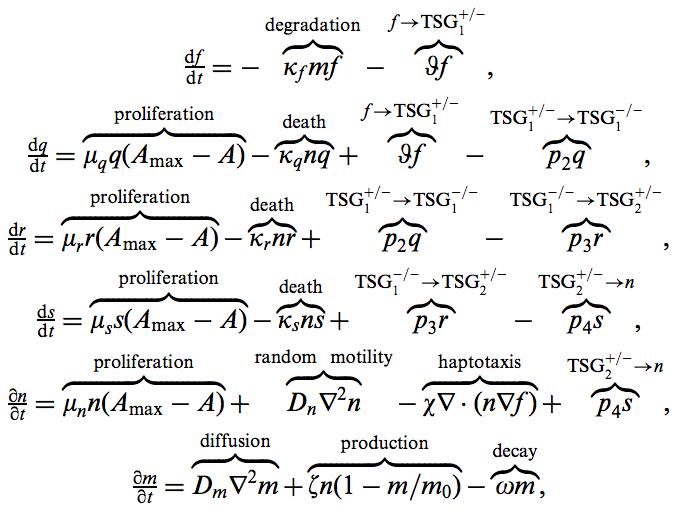
\includegraphics[width=100mm]{pics/Enderling2007}
  \caption{Screenshot from the paper \cite{Enderling:2007uq}. Implemented are 
  only the last two PDEs.}
\end{figure}


\lstset{language=XML}
\begin{lstlisting}
            <!-- PDE: delta n / delta t = ... -->
            <ct:DE type="pde">
                <ct:AssignStatement op="eq">
                    <math:PartialDiff>
                        <math:DiffVariable>
                            <ct:SymbRef symbIdRef="t"/>
                        </math:DiffVariable>
                        <math:DiffOpArgument>
                            <ct:Assign>
                                <ct:SymbRef symbIdRef="n"/>
                            </ct:Assign>
                        </math:DiffOpArgument>
                    </math:PartialDiff>
                    <!-- RHS -->
                    <math:Binop op="plus">
                        <math:Binop op="times">
                            <ct:SymbRef blkIdRef="pm1" symbIdRef="mu_n"/>
                            <math:Binop op="times">
                                <ct:SymbRef symbIdRef="n"/>
                                <math:Binop op="minus">
                                    <ct:SymbRef blkIdRef="pm1" symbIdRef="Amax"/>
                                    <ct:SymbRef blkIdRef="pm1" symbIdRef="A"/>
                                </math:Binop>
                            </math:Binop>
                        </math:Binop>
                        <math:Binop op="plus">
                            <math:Binop op="times">
                                <ct:SymbRef symbIdRef="D_n"/>
                                <math:VectorCalcOp op="laplacian">
                                    <math:DiffVariables>
                                        <ct:Assign>
                                            <ct:SymbRef symbIdRef="x"/>
                                        </ct:Assign>
                                    </math:DiffVariables>
                                    <math:DiffOpArgument>
                                        <ct:Assign>
                                            <ct:SymbRef symbIdRef="n"/>
                                        </ct:Assign>
                                    </math:DiffOpArgument>
                                </math:VectorCalcOp>
                            </math:Binop>
                            <math:Binop op="plus">
                                <math:Uniop op="minus">
                                    <math:Binop op="times">
                                        <ct:SymbRef blkIdRef="pm1" symbIdRef="chi"/>
                                        <math:VectorCalcOp op="divergence">
                                            <math:DiffOpArgument>
                                                <ct:Assign>
                                                    <math:Binop op="times">
                                                        <ct:SymbRef symbIdRef="n"/>
                                                        <math:VectorCalcOp op="gradient">
                                                            <math:DiffVariables>
                                                                <ct:Assign>
                                                                    <ct:SymbRef symbIdRef="x"/>
                                                                </ct:Assign>
                                                            </math:DiffVariables>
                                                            <math:DiffOpArgument>
                                                                <ct:Assign>
                                                                    <ct:SymbRef symbIdRef="f"/>
                                                                </ct:Assign>
                                                            </math:DiffOpArgument>
                                                        </math:VectorCalcOp>
                                                    </math:Binop>
                                                </ct:Assign>
                                            </math:DiffOpArgument>
                                        </math:VectorCalcOp>
                                    </math:Binop>
                                </math:Uniop>
                                <math:Binop op="times">
                                    <ct:SymbRef blkIdRef="pm1" symbIdRef="p4"/>
                                    <ct:SymbRef symbIdRef="s"/>
                                </math:Binop>
                            </math:Binop>
                        </math:Binop>
                    </math:Binop>
                </ct:AssignStatement>
            </ct:DE>
            
            <!-- PDE: delta m / delta t = ... -->
            <ct:DE type="pde">
                <ct:AssignStatement op="eq">
                    <math:Diff>
                        <math:DiffVariable>
                            <ct:SymbRef symbIdRef="t"/>
                        </math:DiffVariable>
                        <math:DiffOpArgument>
                            <ct:Assign>
                                <ct:SymbRef symbIdRef="m"/>
                            </ct:Assign>
                        </math:DiffOpArgument>
                    </math:Diff>
                    <math:Binop op="plus">
                        <math:Binop op="times">
                            <ct:SymbRef symbIdRef="D_m"/>
                            <math:VectorCalcOp op="laplacian">
                                <math:DiffVariables>
                                    <ct:Assign>
                                        <ct:SymbRef symbIdRef="x"/>
                                    </ct:Assign>
                                </math:DiffVariables>
                                <math:DiffOpArgument>
                                    <ct:Assign>
                                        <ct:SymbRef symbIdRef="m"/>
                                    </ct:Assign>
                                </math:DiffOpArgument>
                            </math:VectorCalcOp>
                        </math:Binop>
                        <math:Binop op="minus">
                            <math:Binop op="times">
                                <ct:SymbRef symbIdRef="xi"/>
                                <math:Binop op="times">
                                    <ct:SymbRef symbIdRef="n"/>
                                    <math:Binop op="minus">
                                        <ct:Real>1</ct:Real>
                                        <math:Binop op="divide">
                                            <ct:SymbRef symbIdRef="m"/>
                                            <ct:SymbRef symbIdRef="m_0"/>
                                        </math:Binop>
                                    </math:Binop>
                                </math:Binop>
                            </math:Binop>
                            <math:Binop op="times">
                                <ct:SymbRef blkIdRef="pm1" symbIdRef="omega"/>
                                <ct:SymbRef symbIdRef="m"/>
                            </math:Binop>
                        </math:Binop>
                    </math:Binop>
                </ct:AssignStatement>
            </ct:DE>
\end{lstlisting}


%\subsection{MATLAB notation for parabolic and elliptic PDEs}
%\label{subsec:MatlabPDE}
%Source:
%\url{http://nl.mathworks.com/help/matlab/math/partial-differential-equations.html}
%
%\bigskip
%General format of parabolic and elliptic PDEs, with ICs and BCs, in one spatial variable x 
%and time t in MATLAB reads:
%\begin{align}
%c \Big(x,t,u,\frac{\partial u}{\partial x}\Big) \frac{\partial u}{\partial t} 
%	&= x^{-m} \frac{\partial}{\partial x}  \Big( x^{m} f\Big(x,t,u,\frac{\partial u}{\partial x}\Big)\Big) + s\Big(x,t,u,\frac{\partial u}{\partial x}\Big) \nonumber \\
%	IC: \quad & u(x,t_0) = u_0(t)\nonumber \\
%	BC: \quad & p(x,t,u) + q(x,t) f\Big(x,t,u,\dfrac{\partial u}{\partial x} \Big) \nonumber 
%\end{align}
%This format is mentioned here as it could be supported as an extension/alternative 
%of the structure described so far. 
%


\subsection{PharmML code}
\label{subsec:PDEPharmMLcode}


All models listed in this section are fully encoded and available
in the release pack: \emph{Advection.xml}, \emph{AdvectionDiffusion.xml},
\emph{capillaryTissueExchange.xml}, \emph{Diffusion\_Ghaffarizadeh.xml}, 
\emph{Diffusion.xml}, \emph{Enderling2007.xml}, \emph{SchnakenbergSystem.xml}, 
\emph{ReactionDiffusion.xml}, \emph{Heat.xml}.









%%%%%%%%%%%%%%%%%%%%%%%%%%%%%%%%%%%%%%%%%%%%%%%%%%%%%%%%%%%%%%%%%%%%%%%
%\bigskip
%\subsection{Anderson  Model}
%Source: \cite{}
%
%\subsection*{Model definition}
%
%\begin{figure}[htb]
%\centering
%  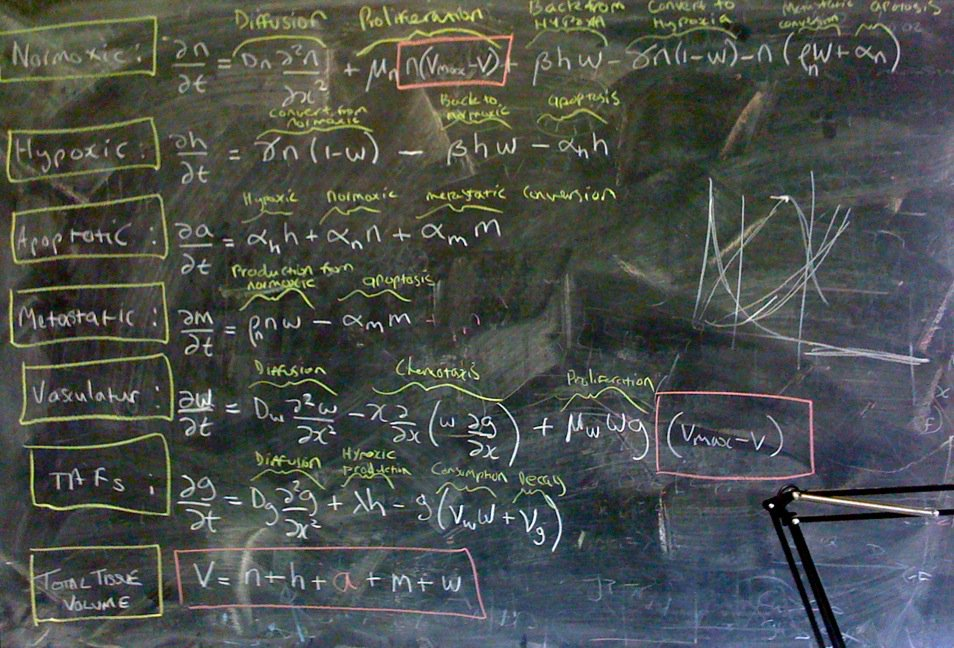
\includegraphics[width=100mm]{pics/Jan29twitte_model}
%  \caption{Screenshot from the Anderson et al. model.}
%\end{figure}
%
%%%%%%%%%%%%%%%%%%%%%%%%%%%%%%%%%%%%%%%%%%%%%%%%%%%%%%%%%%%%%%%%%%%%%%%
%\bigskip
%\subsection{Box 3 | Hybrid models in cancer}
%Source: \cite{}
%
%%%%%%%%%%%%%%%%%%%%%%%%%%%%%%%%%%%%%%%%%%%%%%%%%%%%%%%%%%%%%%%%%%%%%%









